\documentclass[crop,tikz]{standalone}
\usetikzlibrary{backgrounds}
\colorlet{blue}{cyan}
\tikzset{
  inverted/.style = {
    color=white,
    background rectangle/.style={fill},
    show background rectangle
  }
}

\usetikzlibrary{calc}
\tikzset{>=latex}
\colorlet{green}{green}
\colorlet{gray}{gray!60}
\newcommand{\F}{\vec{F}}
\newcommand{\Z}{\vec{Z}}

\begin{document}
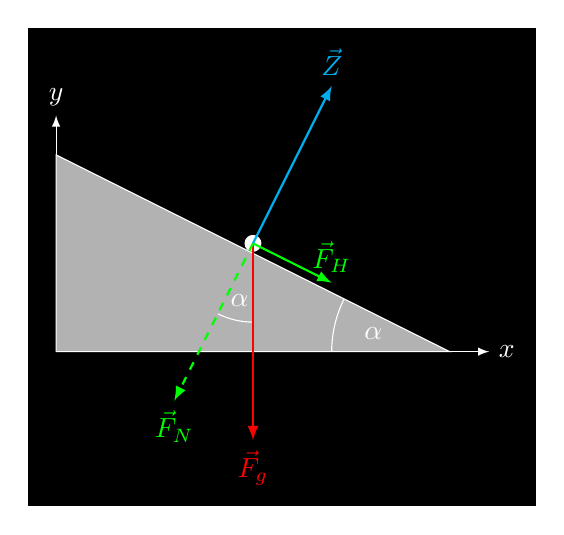
\begin{tikzpicture}[inverted,scale=2.5]
  \pgfmathsetmacro{\al}{atan(0.5)} % angle
  \pgfmathsetmacro{\sa}{sin(\al)}; % sin(angle)
  \pgfmathsetmacro{\ca}{cos(\al)}; % cos(angle)
  % axis
  \draw[->] (0,0) -- ++(2.2,0) node[right] {$x$};
  \draw[->] (0,0) -- ++(0,1.2) node[above] {$y$};
  % inclined plane
  \draw[fill=gray] (0,0) -- (2,0) -- (0,1) -- cycle;
  % position of mass
  \draw[fill,white] (1,0.55) circle (0.04) coordinate (a);
  % arc
  \draw ([shift={({180-\al}:0.6)}]2,0) arc ({180-\al}:180:0.6);
  \node at ($(2,0)+({180-\al/2}:0.4)$) {$\alpha$};
  % arc
  \draw ([shift={(-90:0.4)}]a) arc (-90:{-90-\al}:0.4);
  \node at ($(a)+({-90-\al/2}:0.3)$) {$\alpha$};
  % forces
  \draw[->,thick,red]          (a) -- +(0,-1) node[below] {$\F_g$};
  \draw[->,thick,green]        (a) -- +($(\sa*\ca,-\sa*\sa)$) node[above] {$\F_H$};
  \draw[->,thick,green,dashed] (a) -- +($(-\sa*\ca,-\ca*\ca)$) node[below] {$\F_N$};
  \draw[->,thick,blue]         (a) -- +($(\sa*\ca,\ca*\ca)$) node[above] {$\Z$};
\end{tikzpicture}
\end{document}
